\documentclass[11pt]{article}
\usepackage[T1]{fontenc}
\usepackage[margin=1in]{geometry}
\usepackage{amsmath,amssymb,amsthm,mathtools}
\usepackage{graphicx}
\usepackage{microtype}
\usepackage{xcolor}
\usepackage[colorlinks=true,linkcolor=blue!60!black,urlcolor=blue!70!black,citecolor=blue!60!black]{hyperref}

\newtheorem{theorem}{Theorem}
\newtheorem{corollary}[theorem]{Corollary}
\newtheorem{proposition}[theorem]{Proposition}
\newcommand{\HH}{\mathcal H}
\newcommand{\ellJ}{\ell^2(J)}

\title{Frames with diagonal frame operator:\\exact operator and perturbation parametrizations}
\author{Candidate full solution to two explicit questions in arXiv:2309.06331}
\date{11 August 2026}

\begin{document}
\maketitle

\noindent
\fbox{\begin{minipage}{0.94\textwidth}
\textbf{Status: candidate full solution, likely valid.}
Fix the orthonormal basis with respect to which \emph{diagonal} is meant. If a
frame has frame operator \(S\), then all bounded operators producing a
diagonal-frame-operator frame are exactly
\[
 M=D^{1/2}CS^{-1/2},
\]
where \(D\) is positive, invertible, and diagonal and \(C\) is a coisometry.
All additive perturbations are likewise exactly
\[
 d_j=D^{1/2}Ce_j-v_j.
\]
These formulas hold in finite and infinite dimensions. The packet also
settles the source's canonical-dual boundedness question and gives a sharp
minimax characterization of componentwise perturbation radii that preserve
all frames with a prescribed lower bound.
\end{minipage}}

\section{The source questions}

Let \(\{v_j\}_{j\in J}\) be a frame in a real or complex Hilbert space.
The source asks which operators \(M\) make \(\{Mv_j\}\) a frame whose frame
operator is diagonal, and equivalently which additive perturbations
\(\{d_j\}\) make \(\{v_j+d_j\}\) such a frame \cite[p.~11]{AGR}. The full
source page is reproduced below.

\begin{center}
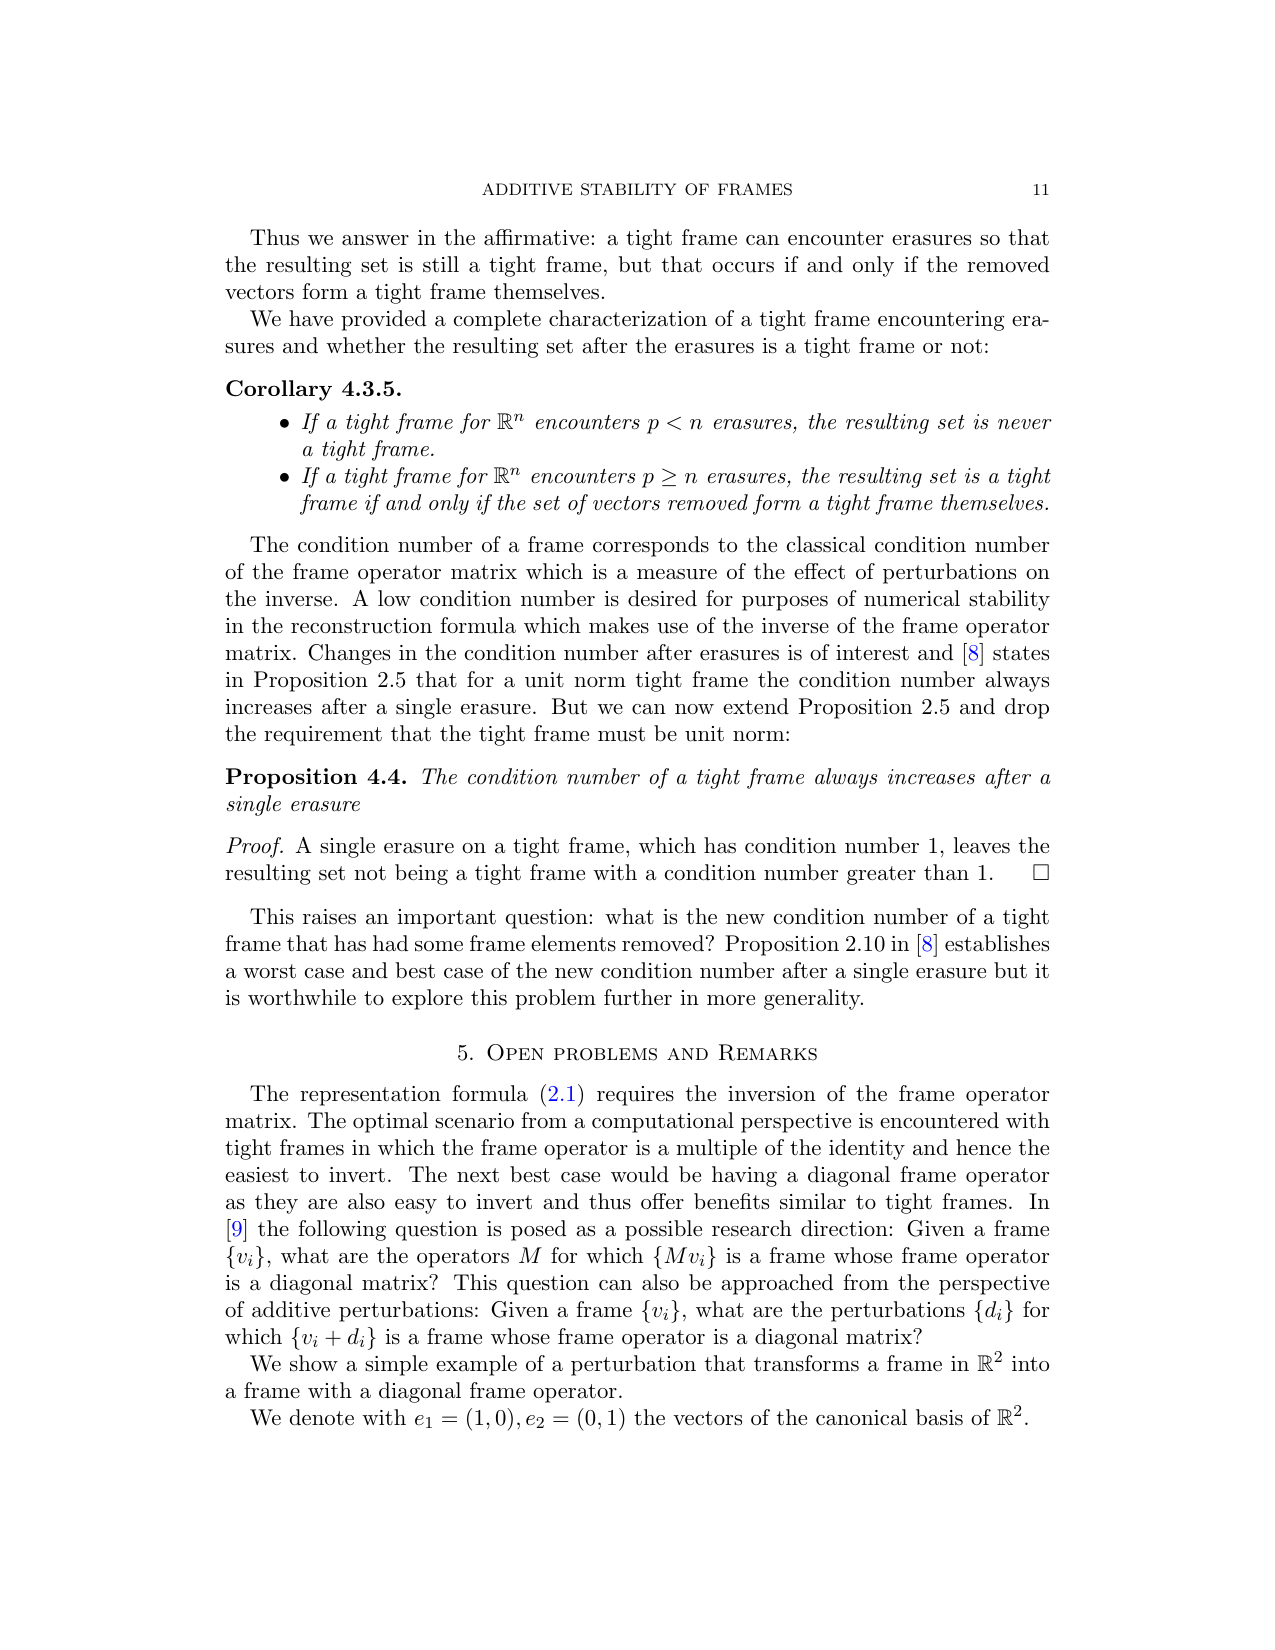
\includegraphics[height=0.69\textheight]{figures/source_open-11.png}
\end{center}

The next page asks how far a frame must be perturbed to obtain a diagonal
frame operator. It then turns to infinite dimensions, observing that the
boundedness of the canonical dual is not immediately obvious, and asks for
the perturbation radii in the Krein--Milman--Rutman setting that preserve
frames \cite[p.~12]{AGR}.

\begin{center}
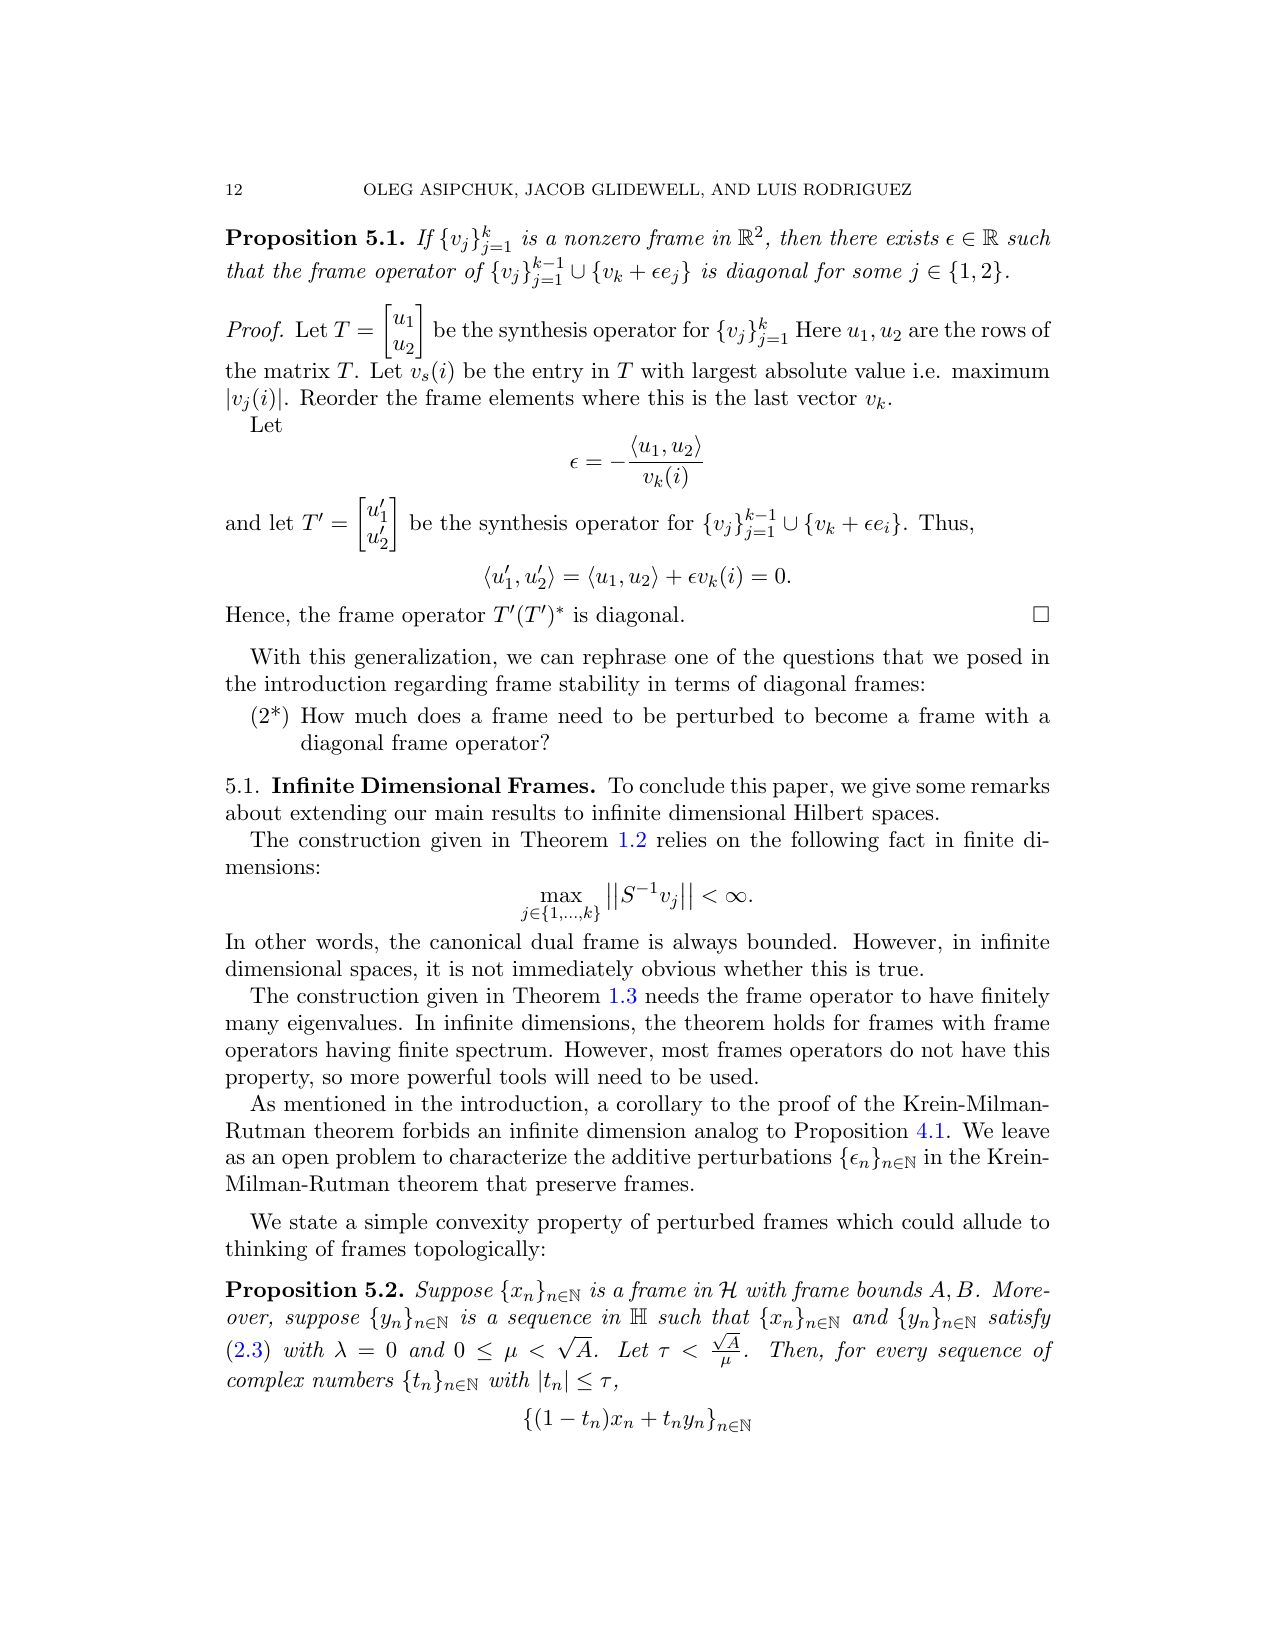
\includegraphics[height=0.78\textheight]{figures/source_open-12.png}
\end{center}

\section{Setup and proof intuition}

Let \(T:\ellJ\to\HH\) be the synthesis operator, \(Te_j=v_j\). The frame
operator is \(S=TT^*\), and the frame condition is exactly that \(S\) is
positive and boundedly invertible. There are then only two identities to
use:
\[
 \text{frame operator of }\{Mv_j\}=MSM^*,
 \qquad
 \text{frame operator of }\{We_j\}=WW^*.
\]
Factoring a desired positive diagonal operator \(D\) turns either identity
into \(CC^*=I\). Thus the apparently nonlinear classification is precisely
the elementary parametrization of factorizations of \(D\) through a
coisometry.

Throughout, diagonal operators are diagonal relative to a fixed orthonormal
basis of \(\HH\). A \emph{coisometry} \(C:\mathcal K\to\HH\) means
\(CC^*=I_{\HH}\). Positive invertibility of a diagonal operator includes
uniform lower and upper bounds on its diagonal entries.

\section{Complete operator classification}

\begin{theorem}[operator parametrization]\label{thm:operator}
Let \(\{v_j\}_{j\in J}\) be a frame for \(\HH\), with frame operator \(S\).
For \(M\in\mathcal B(\HH)\), the following are equivalent.
\begin{enumerate}
\item The family \(\{Mv_j\}_{j\in J}\) is a frame and its frame operator is
diagonal.
\item There are a positive invertible diagonal operator \(D\) on \(\HH\)
and a coisometry \(C:\HH\to\HH\) such that
\[
 M=D^{1/2}CS^{-1/2}.
\]
\end{enumerate}
For a specified resulting frame operator \(D\), this describes all such
\(M\). In finite dimensions \(C\) is unitary (orthogonal over the reals).
\end{theorem}

\begin{proof}
The transformed synthesis operator is \(MT\), so its frame operator is
\(MSM^*\). Suppose first that this is a positive invertible diagonal
operator \(D\), and define
\[
 C=D^{-1/2}MS^{1/2}.
\]
Then
\[
 CC^*=D^{-1/2}MSM^*D^{-1/2}=I,
\]
and rearrangement gives the asserted formula for \(M\).

Conversely, if \(M=D^{1/2}CS^{-1/2}\) and \(CC^*=I\), then
\[
 MSM^*=D^{1/2}CC^*D^{1/2}=D.
\]
This operator is positive and boundedly invertible, so \(\{Mv_j\}\) is a
frame with diagonal frame operator \(D\). If \(\HH\) is finite-dimensional,
a square coisometry is unitary.
\end{proof}

The coisometry cannot in general be replaced by a unitary in infinite
dimensions: the backward shift on \(\ell^2(\mathbb N)\) is a noninjective
coisometry. The formula correctly allows \(M\) to be surjective without
being injective.

\section{Complete additive classification}

\begin{theorem}[additive parametrization]\label{thm:additive}
Let \(T:\ellJ\to\HH\) synthesize the frame \(\{v_j\}_{j\in J}\). A sequence
\(\{d_j\}_{j\in J}\subset\HH\) has the property that
\(\{v_j+d_j\}_{j\in J}\) is a frame with diagonal frame operator if and only
if there are a positive invertible diagonal \(D\in\mathcal B(\HH)\) and a
coisometry \(C:\ellJ\to\HH\) such that
\[
 \boxed{\quad d_j=D^{1/2}Ce_j-v_j\quad(j\in J).\quad}
\]
The resulting frame operator is exactly \(D\).
\end{theorem}

\begin{proof}
Put \(w_j=v_j+d_j\). If \(\{w_j\}\) is a frame, its synthesis operator
\(W:\ellJ\to\HH\) is bounded. Its frame operator is \(WW^*\). If \(WW^*=D\)
is positive, invertible, and diagonal, then
\[
 C=D^{-1/2}W
 \quad\text{satisfies}\quad
 CC^*=D^{-1/2}WW^*D^{-1/2}=I.
\]
Thus \(W=D^{1/2}C\), and evaluation at \(e_j\) gives the displayed formula.
The converse follows at once from
\(WW^*=D^{1/2}CC^*D^{1/2}=D\).
\end{proof}

This also yields an entrywise criterion. Let \(\{h_k\}_{k\in K}\) be the
fixed orthonormal basis of \(\HH\), and put
\[
 r_k=W^*h_k=(\langle h_k,w_j\rangle)_{j\in J}\in\ellJ.
\]
Then \(WW^*\) is diagonal exactly when the rows \(r_k\) are pairwise
orthogonal. The family is a frame exactly when, in addition,
\[
 0<\inf_{k\in K}\|r_k\|^2
 \le \sup_{k\in K}\|r_k\|^2<\infty.
\]
Hence Theorem~\ref{thm:additive} is equivalently a complete orthogonal-row
characterization.

\begin{corollary}[an explicit diagonalizing perturbation]\label{cor:tighten}
Every frame can be additively perturbed to a Parseval frame, hence to one
with diagonal frame operator, by
\[
 d_j=(S^{-1/2}-I)v_j.
\]
If \(E=(S^{-1/2}-I)T\) is the synthesis perturbation, then
\[
 EE^*=(S^{1/2}-I)^2,
 \qquad
 \|E\|=\|S^{1/2}-I\|.
\]
In finite dimension the total squared displacement is
\[
 \sum_j\|d_j\|^2
 =\operatorname{tr}(S)-2\operatorname{tr}(S^{1/2})+\dim\HH.
\]
\end{corollary}

\begin{proof}
The new synthesis operator is \(W=S^{-1/2}T\), and \(WW^*=I\). Also
\(EE^*=(S^{-1/2}-I)S(S^{-1/2}-I)=(S^{1/2}-I)^2\). Taking operator norms
proves the second formula, and taking the trace proves the finite-dimensional
identity.
\end{proof}

The corollary supplies an exact cost for this canonical construction; it
does not assert that this is the closest frame among all frames having an
arbitrary diagonal frame operator.

\section{Two infinite-dimensional consequences}

\begin{proposition}[the canonical dual is uniformly bounded]\label{prop:dual}
If \(\{v_j\}\) has frame bounds \(A,B\), then its canonical dual
\(\{S^{-1}v_j\}\) is a frame with bounds \(1/B,1/A\). Consequently
\[
 \sup_j\|S^{-1}v_j\|\le A^{-1/2}.
\]
This estimate is sharp.
\end{proposition}

\begin{proof}
The canonical dual has synthesis operator \(S^{-1}T\) and frame operator
\(S^{-1}TT^*S^{-1}=S^{-1}\). Since \(AI\le S\le BI\), functional calculus
gives \(B^{-1}I\le S^{-1}\le A^{-1}I\). A Bessel family with bound \(1/A\)
has each vector of norm at most \(A^{-1/2}\). Equality holds for the scaled
orthonormal basis \(v_j=\sqrt A\,e_j\).
\end{proof}

The next theorem gives a sharp universal version of the source's
perturbation-radius question. It separates a guarantee based only on the
original lower frame bound and the radii from the subtler question for one
fixed frame.

\begin{theorem}[sharp universal componentwise radii]\label{thm:radii}
Fix \(A>0\) and nonnegative finite radii
\(\varepsilon=(\varepsilon_j)_{j\in J}\), where \(J\) is finite or countable.
The following are equivalent.
\begin{enumerate}
\item For every Hilbert-space frame \(\{v_j\}_{j\in J}\) with lower frame
bound at least \(A\), every sequence satisfying
\(\|d_j\|\le\varepsilon_j\) leaves \(\{v_j+d_j\}\) a frame.
\item \(\varepsilon\in\ell^2(J)\) and
\(\|\varepsilon\|_2<\sqrt A\).
\end{enumerate}
When (2) holds and the original upper bound is \(B\), every such perturbed
frame has bounds
\[
 (\sqrt A-\|\varepsilon\|_2)^2,
 \qquad
 (\sqrt B+\|\varepsilon\|_2)^2.
\]
\end{theorem}

\begin{proof}
Let \(E:\ellJ\to\HH\) be the synthesis perturbation, \(Ee_j=d_j\). If
\(\delta=\|\varepsilon\|_2<\infty\), then for finitely supported \(c\),
\[
 \|Ec\|\le\sum_j|c_j|\varepsilon_j\le\delta\|c\|_2,
\]
so \(\|E\|\le\delta\). For the original synthesis operator \(T\), the
standard synthesis form of the frame inequalities gives
\[
 \|(T+E)^*x\|_2\ge(\sqrt A-\delta)\|x\|,
 \qquad
 \|(T+E)^*x\|_2\le(\sqrt B+\delta)\|x\|.
\]
This proves sufficiency and the asserted bounds.

For necessity, first suppose \(\varepsilon\notin\ell^2(J)\). Given any
frame \(\{v_j\}\), choose a unit vector \(h\) and set
\(d_j=\varepsilon_jh\). The scalar sequence
\((\langle h,v_j\rangle)_j\) lies in \(\ell^2\), while
\((\varepsilon_j)_j\) does not. Hence
\((\langle h,v_j+d_j\rangle)_j\notin\ell^2\), so the new family is not even
Bessel.

Now suppose \(\varepsilon\in\ell^2(J)\) and
\(\delta=\|\varepsilon\|_2\ge\sqrt A\). On \(\ell^2(J)\), take the frame
\(v_j=\sqrt A\,e_j\). Choose a unit vector \(y\) with
\(|\langle y,e_j\rangle|=\varepsilon_j/\delta\), let \(P_y\) be the
orthogonal projection onto \(\mathbb F y\), and put
\[
 d_j=-P_yv_j.
\]
Then \(\|d_j\|=\sqrt A\,\varepsilon_j/\delta\le\varepsilon_j\), but
\(v_j+d_j\in y^\perp\) for every \(j\). The perturbed family is not
complete and hence is not a frame. This proves necessity, including the
boundary \(\delta=\sqrt A\).
\end{proof}

\section{Checks, upgrade attempts, and scope}

\paragraph{Algebra audit.}
All four central assertions reduce to operator identities: \(MSM^*=D\),
\(WW^*=D\), \(S^{-1}SS^{-1}=S^{-1}\), and the norm bound
\(\|E\|\le\|\varepsilon\|_2\). No compactness, spectral discreteness, or
finite-dimensional matrix argument is used.

\paragraph{Deep upgrades.}
The first attempt gave the finite-dimensional formulas with a unitary
factor. The first upgrade identified coisometries as the correct
infinite-dimensional parameter and covered arbitrary countable frames.
The second upgrade extracted the sharp canonical-dual bound. The third
upgrade replaced a one-sided small-perturbation estimate by the exact
minimax threshold in Theorem~\ref{thm:radii}, including counterexamples both
outside \(\ell^2\) and at the boundary. Corollary~\ref{cor:tighten} gives a
fully explicit diagonalizing displacement, but no claim is made that it
minimizes distance to the full nonconvex class of diagonal-frame-operator
frames.

\paragraph{Novelty check.}
Bounded primary-source searches through 11 August 2026 covered the source
title and the phrases \emph{diagonal frame operator}, \emph{frame
perturbation}, \(MSM^*=D\), and coisometric parametrization. The searches
located the source and related work on prescribed/perturbed frame operators,
but no paper explicitly answering the two displayed source questions by
Theorems~\ref{thm:operator} and~\ref{thm:additive}. The factorization is
elementary enough that it may be implicit in standard operator-frame
theory; novelty confidence is therefore moderate rather than high.

\paragraph{Human-review recommendation.}
Check that coisometry, rather than unitarity, is necessary in infinite
dimensions; verify the orthogonal-row equivalence; and audit the two
necessity constructions in Theorem~\ref{thm:radii}.

\begin{thebibliography}{9}
\bibitem{AGR}
O. Asipchuk, J. Glidewell, and L. Rodriguez,
\emph{Additive Stability of Frames},
\href{https://arxiv.org/abs/2309.06331}{arXiv:2309.06331}.

\bibitem{MR}
P. Massey and M. Ruiz,
\emph{Minimization of convex functionals over frame operators};
\href{https://arxiv.org/abs/0710.1258}{arXiv:0710.1258}.
\end{thebibliography}

\end{document}
